\subsection{Classes and Structs}

\begin{itemize}
	\item Objekte werden im Heap erzeugt
	\item Objekte werden mit \textit{new} erzeugt
	\item eine Klasse kann nur von \textit{einer} anderen Klasse erben
	\item eine Klasse kann von \textit{mehreren} interfaces erben
\end{itemize}

\subsubsection{Fields and Constants}

\begin{tabular}{l|l|l}
	\textbf{Field}           & int value = 0;          & - initial is optional                                     \\
	                         &                         & - initialization value must be computable at compile time \\
	                         &                         & - field of a struct must not be initialized               \\ \hline
	\textbf{Constant}        & cons long size = 4;     & - must be initialized                                     \\
	                         &                         & - value must be computable at compile time                \\ \hline
	\textbf{Read-only field} & readonly DateTime date; & - value needs not be computable at compile time           \\
	                         &                         & - value must not be changed later \\
	                         &                         & - must be initialized in their declaration or in a constructor \\
\end{tabular} 

\subsubsection{Parameters}

\textbf{value Parameters}
\begin{multicols}{2}
	\begin{lstlisting}
	void Inc(int x) {x = x + 1;}
	void F() {
		int val = 3;
		Inc(val); // val == 3
	}
	\end{lstlisting}
	\columnbreak
	\begin{itemize}
		\item \textit{call by value}
		\item formal parameter copy of the actual parameter
		\item actual parameter can be an expression
	\end{itemize}
\end{multicols}

\textbf{ref Parameters}
\begin{multicols}{2}
	\begin{lstlisting}
	void Inc(ref int x) { x = x + 1; }
	void F() {
		int val = 3;
		Inc(ref val); // val == 4
	}
	\end{lstlisting}
	\columnbreak
	\begin{itemize}
		\item \textit{call by referenc}
		\item formal parameter is a alias of the actual parameter
		\item actual parameter can be an value
	\end{itemize}
\end{multicols}


\subsubsection{Function Overloading}
\begin{multicols}{2}
\begin{lstlisting}
void F (int x) {...}
void F (char x) {...}
void F (int x, long y) {...}
void F (long x, int y) {...}
void F (ref int x) {...}



int i; long n; short s;
F(i); // F(int x)
F('a'); // F(char x)
F(i, n); // F(int x, long y)
F(n, s); // F(long x, int y);
F(i, s); // ambiguous between F(int x, long y) and F(long x, int y); => compilation error
F(i, i); // ambiguous between F(int x, long y) and F(long x, int y); => compilation error
\end{lstlisting}
	\columnbreak
	Methods of a class may have the same name
	\begin{itemize}
		\item if they have different numbers of parameters, or
		\item if they have different parameter types, or
		\item if they have different parameter kinds (value, ref/out)
	\end{itemize}
\end{multicols}

\subsubsection{Constructor}
\begin{itemize}
	\item Constructors can be overloaded.
	\item A construcor may call another constructor with this
	\item Before a constructor is called, fields are possibly initialized.
\end{itemize}

\begin{multicols}{2}
\begin{lstlisting}
class Rectangle {
	int x, y, width, height;
	public Rectangle (int x, int y, int w, int h) {this.x = x; this.y = y; width = w; height = h; }
	public Rectangle (int w, int h) : this(0, 0, w, h) {}
	public Rectangle () : this(0, 0, 0, 0) {}
	...
}
\end{lstlisting}
\columnbreak
\begin{lstlisting}
Rectangle r1 = new Rectangle();
Rectangle r2 = new Rectangle(2, 5);
Rectangle r3 = new Rectangle(2, 2, 10, 5);
\end{lstlisting}
\end{multicols}

\textbf{Default Constructor}\\ \\
If no constructor was declared in a class, the compiler generates a parameterless default constructor\\
If a constructor was declared, no default constructor is generated\\ 


\textbf{Constructor of Struct}
\begin{itemize}
	\item For every struct the compiler generates a parameterless default constructor (even if there are other constructors).
		  The default constructor zeroes all fields.
	\item A constructor of a struct must initialize all fields.
	\item Programmers must not declare a parameterless constructor for structs (for implementation reasons of the CLR).
\end{itemize}

\begin{multicols}{2}
\begin{lstlisting}
struct Complex {
	double re, im;
	public Complex(double re, double im) { this.re = re; this.im = im; }
	public Complex(double re) : this(re, 0) {}
	...
}
\end{lstlisting}
\columnbreak
\begin{lstlisting}
Complex c0; // c0.re and c0.im uninitialized
Complex c1 = new Complex(); // c1.re == 0, c1.im == 0
Complex c2 = new Complex(5); // c2.re == 5, c2.im == 0
Complex c3 = new Complex(10, 3); // c3.re == 10, c3.im == 3
\end{lstlisting}
\end{multicols}


\textbf{Static Constructor}\\ \\
Gilt für Klassen und Stuct
\begin{itemize}
	\item Must be parameterless (also for structs) and have no public or private modifier.
	\item There must be just one static constructor per class/struct.
	\item Is invoked once before this type is used for the first time.
	\item Used for initialization of static fields.
\end{itemize}

\begin{multicols}{2}
\begin{lstlisting}
class Rectangle {
	...
	static Rectangle() {
	Console.WriteLine("Rectangle initialized");
	}
}
\end{lstlisting}
\columnbreak
\begin{lstlisting}
struct Point {
	...
	static Point() {
	Console.WriteLine("Point initialized");
	}
}
\end{lstlisting}
\end{multicols}

\subsubsection{Destructor}
\begin{itemize}
	\item Correspond to finalizers in Java.
	\item Called for an object before it is removed by the garbage collector.
	\item Can be used, for example, to close open files..
	\item Base class destructor is called automatically at the end.
	\item No public or private.
	\item Structs must not have a destructor
\end{itemize}
\begin{lstlisting}
class Test {
	~Test() {
	... cleanup actions ...
	}
}
\end{lstlisting}

\subsubsection{Properties}
\begin{itemize}
	\item Properties can also be static
	\item Properties work also with assignment operators
	\item \textbf{JIT compilers often inline get/set methods $\rightarrow$ no efficiency penalty. }
\end{itemize}

\begin{figure}[h]
	\centering
	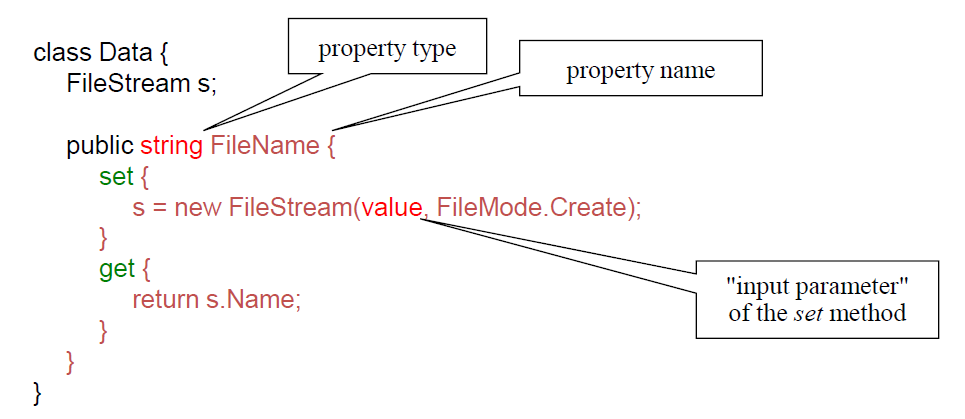
\includegraphics[height=5cm, ]{images/CSharp/Properties}
	\caption{Properties}
\end{figure}

\begin{lstlisting}
Data d = new Data();
d.FileName = "myFile.txt"; // calls set("myFile.txt")
string s = d.FileName; // calls get()
\end{lstlisting}

\textbf{Benefit of properties}
\begin{multicols}{2}
\begin{itemize}
	\item Allow read-only and write-only fields.
	\item Can validate a field when it is accessed.
\end{itemize}
\columnbreak
\begin{itemize}
	\item Interface / implementation of the data can differ.
	\item Substitute for fields in interfaces.
\end{itemize}
\end{multicols}

\subsubsection{Indexer}
\begin{itemize}
	\item get or set method can be omitted (write-only / read-only)
	\item indexers can be overloaded with different index types
	\item .NET library has indexers for string (s[i]), ArrayList (a[i]), etc.
\end{itemize}

\begin{figure}[h]
	\centering
	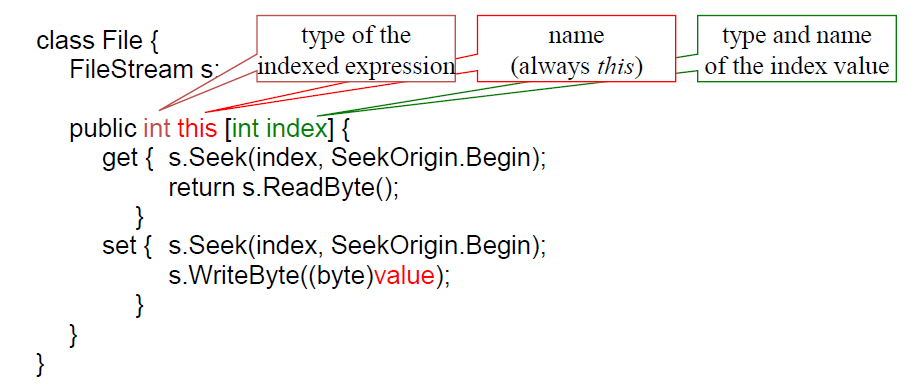
\includegraphics[height=5cm, ]{images/CSharp/Indexer}
	\caption{Indexer}
\end{figure}

\begin{lstlisting}
File f = ...;
int x = f[10]; // calls f.get(10)
f[10] = 'A'; // calls f.set(10, 'A')
\end{lstlisting}

\subsubsection{Operator Overloading}
The following operators can be overloaded:\\
%TODO Zeichen ergänzen 
\begin{tabular}{ll}
	- arithmetic:    & $+, - (unary and binary), *, /, \%, ++, -- $ \\
	- relational:    & $==, !=, <, >, <=, >=$                       \\
	- bit operators: & $\&,|, \text{\textasciicircum}$              \\
	- others:        & $!$ , \textasciitilde, $>>,<>, true, false$  \\
\end{tabular}
\begin{multicols}{2}
\begin{lstlisting}
struct Fraction {
	int x, y;
	public Fraction (int x, int y) { this.x = x; this.y = y; }
	public static Fraction operator + (Fraction a, Fraction b) {
		return new Fraction(a.x * b.y + b.x * a.y, a.y * b.y);
	}
}
\end{lstlisting}
\columnbreak
\begin{lstlisting}
Fraction a = new Fraction(1, 2);
Fraction b = new Fraction(3, 4);
Fraction c = a + b; // c.x == 10, c.y == 8
\end{lstlisting}
\end{multicols}

\subsubsection{Conversion Operators}
\begin{multicols}{2}
\textbf{Implicit conversion}
\begin{itemize}
	\item If the conversion is always possible without loss of precision
	\item e.g. long = int;
\end{itemize}
\columnbreak
\textbf{Explicit conversion}
\begin{itemize}
	\item If a run time check is necessary or truncation is possible
	\item e.g. int = (int) long;
\end{itemize}
\end{multicols}


\begin{lstlisting}
class Fraction {
	int x, y;
	...
	public static implicit operator Fraction (int x) { return new Fraction(x, 1); }
	public static explicit operator int (Fraction f) { return f.x / f.y; }
}
\end{lstlisting}

\begin{lstlisting}
Fraction f = 3; // implicit conversion, f.x == 3, f.y == 1
int i = (int) f; // explicit conversion, i == 3
\end{lstlisting}

\subsubsection{Nested Types}
\begin{multicols}{2}
\begin{lstlisting}
class A {
	private int x;
	B b;
	public void Foo() { b.Bar(); }
	...
	public class B {
		A a;
		public void Bar() { a.x = ...; ... a.Foo(); }
		...
	}
}
\end{lstlisting}
\columnbreak
\begin{lstlisting}
class C {
	A a = new A();
	A.B b = new A.B();
}
\end{lstlisting}
\end{multicols}

For auxiliary classes that should be hidden:
\begin{itemize}
	\item Inner class can access all members of the outer class (even private members).
	\item Outer class can access only public members of the inner class.
	\item Other classes can access an inner class only if it is public.
\end{itemize}
Nested types can also be structs, enums, interfaces and delegates.


